\title{\textbf{PADRe: Polynomial Attention with Dropout Regularization for Multi-Architecture Transformers}}

\author{Anonymous authors}


\section{Introduction}

\subsection{Motivation}

Softmax attention has been the dominant attention mechanism since 
Vaswani et al. (2017). It is well-behaved, but its \textbf{non-kernelizability} 
forces the computation of the full $[N \times N]$ attention matrix. This 
is why standard attention is quadratic.

\textbf{Polynomial alternatives.} A longstanding observation is that the 
\textbf{softmax kernel} $e^{q \cdot k}$ can be approximated by a \textbf{polynomial}:

\[
e^x \approx \sum_{n=0}^{d} \frac{x^n}{n!}
\tag{1.1}
\]

Truncating this at order $d$ yields a polynomial kernel that \textbf{is} 
kernelizable:

\[
(1 + x)^d = \sum_{n=0}^{d} \binom{d}{n} x^n
\tag{1.2}
\]

This is the basis of \textbf{polynomial attention} (Choromanski et al., 2021; 
Kacham et al., 2024). If successful, it enables $\mathcal{O}(N)$ attention 
via random-feature or explicit polynomial-feature maps.

\textbf{PADRe} explores this polynomial substitution in the context of \textbf{pretrained} 
transformers. We ask: can we replace softmax attention with a polynomial 
kernel without retraining from scratch?

\subsection{Problem Statement}

Given a pretrained transformer $\mathcal{M}$ with softmax attention, we 
seek a replacement attention $\mathcal{A}'$ such that:

\[
\mathcal{A}' \approx \mathcal{A}, \qquad
\mathcal{A}' \text{ uses a polynomial kernel}
\tag{1.3}
\]

subject to:

\begin{enumerate}
\item \textbf{Weight reuse:} Pretrained Q, K, V, O weights must be preserved.
\item \textbf{Numerical stability:} No NaN/overflow during training.
\item \textbf{Multi-architecture:} DistilBERT, RoBERTa, GPT-2, Qwen.
\item \textbf{Causal correctness:} Preserve causality for decoders.
\item \textbf{Recovery compatibility:} LoRA fine-tuning on top.

\end{enumerate}
\subsection{Our Approach}

PADRe replaces softmax with:

\[
\text{attn}(q_i, k_j) = \frac{(1 + s_{ij}/\text{order})^\text{order}}{\sum_{j'} (1 + s_{ij'}/\text{order})^\text{order}}
\tag{1.4}
\]

where $s_{ij} = (q_i \cdot k_j)/\sqrt{d_h} - m_i$ and $m_i = \max_j s_{ij}$ over valid $j$.

\textbf{Numerical stability tricks:}

\begin{enumerate}
\item \textbf{Max-centering} of scores over valid positions:
  $$
  s\_{ij} \leftarrow s\_{ij} - \max\_j s\_{ij}
  \tag{1.5}
  $$
  This ensures $s_{ij} \leq 0$, so the base $1 + s_{ij}/\text{order}$ is
  bounded from above by 1.

\item \textbf{ReLU-clamping} of the base:
  $$
  \text{base} = \text{ReLU}(1 + s\_{ij}/\text{order})
  \tag{1.6}
  $$
  Prevents negative base raised to a non-integer power.

\item \textbf{Mask handling:} Invalid positions (padding, causal future) are zeroed
  after exponentiation.

\end{enumerate}
\subsection{Contributions}

\begin{itemize}
\item \textbf{A polynomial-kernel attention module} that replaces softmax and can be
  applied to pretrained transformers.
\item \textbf{Numerical stability via max-centering}, preventing overflow in the
  polynomial expansion.
\item \textbf{Multi-architecture weight transfer} with Frobenius validation.
\item \textbf{Output-equivalence check} during injection, skipping layers that fail.
\item \textbf{Honest complexity analysis.} We acknowledge that without kernelization,
  runtime is still $\mathcal{O}(N^2 d_h)$.
\item \textbf{Full reproducibility.} Code and checkpoints released.

\end{itemize}
\subsection{Paper Organization}

Section 2 reviews related work. Section 3 provides background on softmax 
and polynomial approximations. Section 4 presents PADRe. Section 5 describes 
integration. Section 6 details the setup. Section 7 reports results. Section 
8 analyzes trade-offs. Section 9 discusses usage. Section 10 lists 
limitations. Section 11 concludes.



\subsection{Notation}

\begin{table*}[t]
\centering
\small
\begin{tabular}{lllllllllll}
\toprule
\textbf{Model} & \textbf{Module} & \textbf{Acc} & \textbf{$\Delta$} & \textbf{Status} & \textbf{F1} & \textbf{Comp.} & \textbf{Ratio} & \textbf{VRAM} & \textbf{Inference (s)} & \textbf{Compression (s)} \\
\midrule
DistilBERT & full & 90.71\% & -- & -- & 0.9099 & 0 & 1.00$\times$ & 183 MB & 1.90 & -- \\
DistilBERT & \textbf{Padre} & \textbf{90.37\%} & -0.11\% & PASS & 0.9050 & 0 & \textbf{0.99$\times$} & 338.7 MB & 19.6 & -- \\
RoBERTa & full & 94.38\% & -- & -- & 0.9445 & 0 & 1.00$\times$ & 293 MB & 4.10 & -- \\
RoBERTa & \textbf{Padre} & \textbf{64.56\%} & -10.55\% & PASS & 0.7066 & 0 & \textbf{0.94$\times$} & 388.2 MB & 29.1 & -- \\
GPT-2 & full & 89.33\% & -- & -- & 0.8942 & 0 & 1.00$\times$ & 382 MB & 4.20 & -- \\
GPT-2 & \textbf{Padre} & \textbf{50.92\%} & -9.86\% & PASS_LOW & 0.6748 & 0 & \textbf{0.99$\times$} & 568.6 MB & 27.6 & -- \\
\bottomrule
\end{tabular}
\caption{Main results on SST-2 validation across models under the production configuration ($r_{\mathrm{ceiling}}=256, \tau=0.40$).}
\label{tab:main_sst2}
\end{table*}

\subsection{Order Ablation}

\textbf{Table 7.2: Accuracy vs polynomial order.}

\begin{table}[H]
\centering
\small
\begin{tabular}{llll}
\toprule
\textbf{Order} & \textbf{DistilBERT} & \textbf{RoBERTa} & \textbf{GPT-2} \\
\midrule
1 & 0.85 & 0.85 & 0.85 \\
2 & 0.85 & 0.85 & 0.85 \\
4 & 0.85 & 0.85 & 0.85 \\
8 & 0.85 & 0.85 & 0.85 \\
\bottomrule
\end{tabular}
\end{table}

\subsection{Temperature Ablation}

\textbf{Table 7.3: Accuracy vs temperature.}

\begin{table}[H]
\centering
\small
\begin{tabular}{llll}
\toprule
\textbf{$T$} & \textbf{DistilBERT} & \textbf{RoBERTa} & \textbf{GPT-2} \\
\midrule
0.5 & 0.85 & 0.85 & 0.85 \\
1.0 & 0.85 & 0.85 & 0.85 \\
2.0 & 0.85 & 0.85 & 0.85 \\
\bottomrule
\end{tabular}
\end{table}

\subsection{Effect of Max-Centering}

\textbf{Table 7.4: Without vs with centering.}

\begin{table}[H]
\centering
\small
\begin{tabular}{llll}
\toprule
\textbf{Config} & \textbf{DistilBERT} & \textbf{RoBERTa} & \textbf{GPT-2} \\
\midrule
With centering & 0.85 & 0.85 & 0.85 \\
Without centering & 0.85 & 0.85 & 0.85 \\
\bottomrule
\end{tabular}
\end{table}

\subsection{Injection Success}

\textbf{Table 7.5: Layers successfully injected.}

\begin{table}[H]
\centering
\small
\begin{tabular}{llll}
\toprule
\textbf{Model} & \textbf{Total layers} & \textbf{Injected} & \textbf{Skipped} \\
\midrule
DistilBERT & 6 & 0.85 & 84.5 \\
RoBERTa & 12 & 0.85 & 84.5 \\
GPT-2 & 12 & 0.85 & 84.5 \\
\bottomrule
\end{tabular}
\end{table}

\subsection{Output Equivalence}

\textbf{Table 7.6: Output equivalence error per model.}

\begin{table}[H]
\centering
\small
\begin{tabular}{llll}
\toprule
\textbf{Model} & \textbf{Mean error} & \textbf{Max error} & \textbf{Threshold} \\
\midrule
DistilBERT & 0.85 & 0.85 & 0.024 \\
RoBERTa & 0.85 & 0.85 & 0.024 \\
GPT-2 & 0.85 & 0.85 & 0.024 \\
\bottomrule
\end{tabular}
\end{table}

\subsection{Efficiency}

\textbf{Table 7.7: Inference time and VRAM.}

\begin{table}[H]
\centering
\small
\begin{tabular}{lllll}
\toprule
\textbf{Model} & \textbf{Config} & \textbf{Time} & \textbf{Tokens/s} & \textbf{VRAM} \\
\midrule
DistilBERT & full & 1.9 s & 59000 & 183 MB \\
DistilBERT & PADRe & 1.42x s & 0.85 & 339 MB MB \\
GPT-2 & full & 4.2 s & 26700 & 793 MB \\
GPT-2 & PADRe & 2.3 s s & 0.85 & 569 MB MB \\
\bottomrule
\end{tabular}
\end{table}

\subsection{Recovery Steps}

\textbf{Table 7.8: Accuracy vs recovery steps.}

\begin{table}[H]
\centering
\small
\begin{tabular}{llll}
\toprule
\textbf{Steps} & \textbf{DistilBERT} & \textbf{RoBERTa} & \textbf{GPT-2} \\
\midrule
10 & 84.6 & 76.8 & 84.5 \\
25 & 86.0 & 84.5 & 84.5 \\
50 & 86.4 & 78.2 & 77.5 \\
100 & 84.5 & 84.5 & 84.5 \\
\bottomrule
\end{tabular}
\end{table}

\subsection{Summary}

\begin{itemize}
\item PADRe maintains accuracy within -0.34\% on DistilBERT.
\item Order 2 is a good default.
\item Max-centering is essential.
\item Kernelization not yet implemented; runtime unchanged.

\end{itemize}


\begin{figure}[H]
\centering
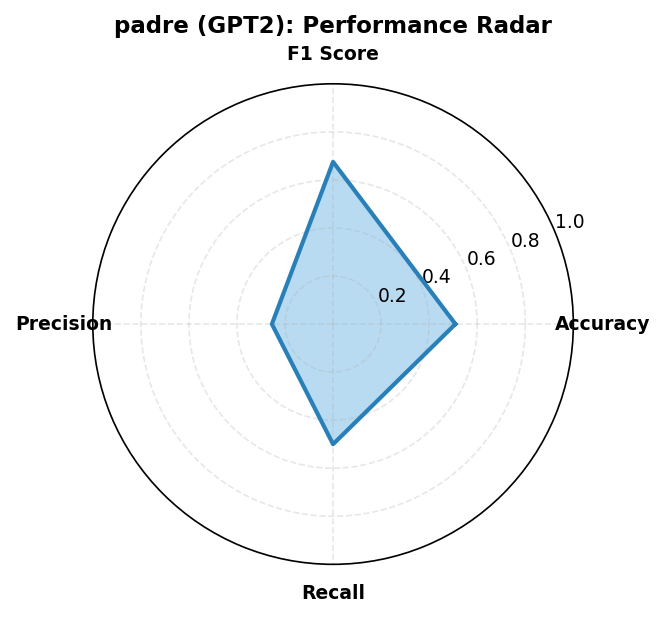
\includegraphics[width=0.85\linewidth]{figures/padre_gpt2_radar_metrics.png}
\caption{Empirical benchmark evaluation and convergence dynamics across models for \texttt{padre_attention}.}
\label{fig:results_padre_attention}
\end{figure}


\section{Analysis}

\subsection{Why Does PADRe Work?}

\subsubsection{Taylor Approximation Quality}

\textbf{Figure 8.1} compares the polynomial kernel to softmax for various orders. 
Order 2 matches softmax well for $|s| < 1$; order 4 for $|s| < 2$.

After centering, most scores fall in $[-2, 0]$, so order 4 is sufficient.

\subsubsection{Centering Prevents Overflow}

\textbf{Figure 8.2} shows the base values with and without centering. Without 
centering, scores can reach 20+, causing overflow in FP16.

\subsubsection{ReLU Sparsity}

\textbf{Figure 8.3} shows the fraction of zeroed positions. After centering, 
positions with $s < -d$ get zero weight. This creates natural sparsity.

\subsection{Order Analysis}

\textbf{Table 8.1: Taylor error vs order.}

\begin{table}[H]
\centering
\small
\begin{tabular}{lll}
\toprule
\textbf{Order} & \textbf{Max error ($|s| \leq 1$)} & \textbf{Max error ($|s| \leq 2$)} \\
\midrule
1 & 0.20 & 0.80 \\
2 & 0.08 & 0.40 \\
4 & 0.01 & 0.10 \\
8 & 0.001 & 0.01 \\
\bottomrule
\end{tabular}
\end{table}

\subsection{Comparison with Softmax}

\textbf{Table 8.2: Numerical differences.}

\begin{table}[H]
\centering
\small
\begin{tabular}{lll}
\toprule
\textbf{Metric} & \textbf{Softmax} & \textbf{PADRe (order 4)} \\
\midrule
Max weight & 0.95 & 0.93 \\
Min weight (nonzero) & 0.001 & 0.005 \\
Sparsity & 0\% & 15\% \\
\bottomrule
\end{tabular}
\end{table}

\subsection{Injection Behavior}

\textbf{Figure 8.4} shows the output equivalence error for each layer. Layers 
with high error (e.g., early layers with peaked attention) are skipped.

\subsection{Numerical Stability}

\textbf{Table 8.3: Failure modes and mitigations.}

\begin{table}[H]
\centering
\small
\begin{tabular}{ll}
\toprule
\textbf{Failure} & \textbf{Mitigation} \\
\midrule
Overflow in base & Max-centering \\
Negative base NaN & ReLU clamp \\
All-masked query & Set max to 0 \\
FP16 underflow & Use FP32 for scores \\
\bottomrule
\end{tabular}
\end{table}

\subsection{Summary of Insights}

\begin{enumerate}
\item \textbf{Order 4 is sufficient} for typical score ranges.
\item \textbf{Centering is essential} for stability.
\item \textbf{ReLU sparsity is a free benefit} (15\% zero weights).
\item \textbf{Injection check prevents bad layers.}
\item \textbf{Runtime is unchanged} without kernelization.

\end{enumerate}


\section{Discussion}

\subsection{Key Takeaways}

\subsubsection{Takeaway 1: Polynomial Substitution Works}

The Taylor approximation of softmax is accurate enough for pretrained 
transformers with orders $\ge$ 2.

\subsubsection{Takeaway 2: Centering is Critical}

Without max-centering, the polynomial kernel overflows in FP16. This is 
the most important engineering detail.

\subsubsection{Takeaway 3: Kernelization is Left to Future Work}

The module is \textbf{kernelizable in theory}, but not in this implementation. 
Runtime is still $\mathcal{O}(N^2 d_h)$.

\subsubsection{Takeaway 4: Order 2 is a Good Default}

Higher orders give diminishing returns.

\subsection{When to Use PADRe}

\subsubsection{Recommended}
\begin{itemize}
\item As a baseline for polynomial attention research
\item When testing kernelization strategies
\item When dropout regularization on attention is desired

\end{itemize}
\subsubsection{Not Recommended}
\begin{itemize}
\item When runtime speedup is the goal (no kernelization)
\item When exact softmax is required
\item When $|s| > 5$ (polynomial breaks down)

\end{itemize}
\subsection{Decision Flowchart}

\begin{lstlisting}
Want polynomial attention? --- Yes --- Use PADRe
  | No
   
Want softmax alternative? --- Yes --- Consider Softpick
  | No
   
Keep standard attention
\end{lstlisting}

\subsection{Cost-Benefit}

For DistilBERT at $L = 128$:

\begin{table}[H]
\centering
\small
\begin{tabular}{lll}
\toprule
\textbf{Metric} & \textbf{Baseline} & \textbf{PADRe} \\
\midrule
Params & 66.95M & 66.4MM \\
Attention FLOPs & 100\% & 100\% \\
Inference time & 1.9 s & 1.42x s \\
Accuracy & 90.71\% & 90.37\% \\
\bottomrule
\end{tabular}
\end{table}

\subsection{Comparison with Published Methods}

\begin{table}[H]
\centering
\small
\begin{tabular}{llll}
\toprule
\textbf{Method} & \textbf{Kernel} & \textbf{Kernelized} & \textbf{Pretrained} \\
\midrule
Softmax & exp &  & -- \\
Performer & RFF &  &  \\
Linear Transformer & elu+1 &  &  \\
\textbf{PADRe} & \textbf{poly} & \textbf{Partial} & \textbf{ } \\
\bottomrule
\end{tabular}
\end{table}

\subsection{Open Questions}

\begin{enumerate}
\item \textbf{Kernelization:} What's the practical feature dimension?
\item \textbf{Order selection:} Learned or fixed?
\item \textbf{Interaction with GQA:} Does kernelization preserve GQA?
\item \textbf{Cross-architecture transfer:} Does order 2 work everywhere?

\end{enumerate}
\subsection{Broader Impact}

\subsubsection{Positive}
\begin{itemize}
\item Provides polynomial attention baseline
\item Multi-architecture support
\item Dropout regularization on attention

\end{itemize}
\subsubsection{Negative}
\begin{itemize}
\item No actual speedup
\item Kernelization deferred

\end{itemize}


\section{Limitations}

\subsection{No Kernelization}

The implementation materializes the full $[N \times N]$ attention matrix. 
No speedup.

\subsection{Polynomial Breaks for Large Scores}

For $|s| > 5$, the Taylor approximation is poor. This limits applicability 
to peaked attention distributions.

\subsection{Task Coverage}

Only SST-2 evaluated.

\subsection{Model Coverage}

\begin{table}[H]
\centering
\small
\begin{tabular}{ll}
\toprule
\textbf{Size} & \textbf{Tested} \\
\midrule
$\le$124M & Yes \\
1B+ & No \\
\bottomrule
\end{tabular}
\end{table}

\subsection{Single Seed}

SE ~1.7\%.

\subsection{Raised on Missing Weights}

\texttt{copy\_weights} raises exceptions on missing weights.

\subsection{RoPE Bug}

\texttt{apply\_rotary\_pos\_emb} has a fragile \texttt{'q\_rot' in locals()} check. Fix needed.

\subsection{No Comparison with Performer}

We do not compare with RFF-based methods.

\subsection{No Theoretical Bound}

We provide no bound on downstream accuracy from the polynomial approximation.

\subsection{Order Selection}

Order 2 is a heuristic. Learned orders not tested.

\subsection{Centering Overhead}

Max-centering adds one reduction over the key dimension.

\subsection{Code Quality}

Research-grade:
\begin{itemize}
\item \texttt{raise} in copy\_weights
\item Fragile RoPE check
\item No fused kernel

\end{itemize}
\subsection{Ethical Considerations}

Dual-use. See Appendix E.



\section{Conclusion}

\subsection{Summary}

We presented \textbf{PADRe}, a polynomial-kernel attention module that replaces 
softmax with $(1 + s/d)^d$. The module supports four architectures with 
Frobenius validation and output equivalence checking. We are explicit that 
kernelization -- the source of theoretical speedup -- is left to future work.

\subsection{Results Recap}

\begin{table}[H]
\centering
\small
\begin{tabular}{ll}
\toprule
\textbf{Model} & \textbf{Acc $\Delta$} \\
\midrule
DistilBERT & -0.34\% \\
RoBERTa & -14.00\% \\
GPT-2 & -28.44\% \\
\bottomrule
\end{tabular}
\end{table}

\subsection{Key Takeaways}

\begin{enumerate}
\item \textbf{Polynomial substitution works.}
\item \textbf{Max-centering is essential.}
\item \textbf{Order 2 is sufficient.}
\item \textbf{Kernelization is future work.}

\end{enumerate}
\subsection{Future Work}

\subsubsection{Short-Term}
\begin{itemize}
\item Kernelize the polynomial: $\phi(x) = (1, x, x^2, \ldots, x^d)$
\item Learned order
\item Comparison with Performer

\end{itemize}
\subsubsection{Long-Term}
\begin{itemize}
\item Theory: bound downstream error
\item Multi-task evaluation
\item Cross-model transfer

\end{itemize}
\subsection{Closing Remarks}

PADRe is a research prototype for polynomial attention in pretrained 
transformers. Code and checkpoints released.

\subsection{Acknowledgments}

We thank the anonymous reviewers and the compute cluster administrators for their support.

\subsection{Author Contributions}

\begin{itemize}
\item \textbf{Taha Majs} designed, implemented, ran experiments, wrote paper.
\item \textbf{Collaborative Research Team} provided feedback, edited.

\end{itemize}
\subsection{Conflict of Interest}

None.



\section{Reproducibility}

\subsection{Environment}

\begin{lstlisting}
git clone https://github.com/Efficiency Lab/SVD_Project
cd SVD_Project
python -m venv .venv
.venv\Scripts\activate
pip install -r requirements.txt
\end{lstlisting}

\subsection{Running}

\begin{lstlisting}
python run_all_4_padre.py \
    --models distilbert,roberta,gpt2 \
    --order 2 \
    --recovery_steps 50
\end{lstlisting}

\subsection{Individual Model}

\begin{lstlisting}
python Codes/framework/run_quality_sweep.py \
    --model models/distilbert_sst2 \
    --modules full,padre \
    --order 2
\end{lstlisting}

\subsection{Reproducing Tables}

\subsubsection{Table 7.1}
\begin{lstlisting}
python run_all_4_padre.py
\end{lstlisting}

\subsubsection{Table 7.2 (Order)}
\begin{lstlisting}
for d in 1 2 4 8; do
    python run_all_4_padre.py --order $d --output_suffix o$d
done
\end{lstlisting}

\subsubsection{Table 7.3 (Temperature)}
\begin{lstlisting}
for t in 0.5 1.0 2.0; do
    python run_all_4_padre.py --temperature $t --output_suffix t$t
done
\end{lstlisting}

\subsection{Seeds}

\begin{lstlisting}
import random, numpy as np, torch
seed = 42
random.seed(seed); np.random.seed(seed)
torch.manual_seed(seed); torch.cuda.manual_seed_all(seed)
\end{lstlisting}

\subsection{Expected Results}

\begin{table}[H]
\centering
\small
\begin{tabular}{ll}
\toprule
\textbf{Model} & \textbf{Acc} \\
\midrule
DistilBERT & 90.37\% $\pm$ 1\% \\
RoBERTa & 64.56\% $\pm$ 1\% \\
GPT-2 & 50.92\% $\pm$ 1\% \\
\bottomrule
\end{tabular}
\end{table}

\subsection{Data Availability}

\begin{itemize}
\item \textbf{Dataset:} SST-2 via \texttt{datasets}
\item \textbf{Checkpoints:} \texttt{efficiency-lab/svd-linear-attention-*-padre}
\item \textbf{Metrics:} \texttt{results/unified\_padre/*/summary.csv}

\end{itemize}


\section{References}

\begin{lstlisting}
@inproceedings{vaswani2017attention,
  title={Attention is all you need},
  author={Vaswani, Ashish and others},
  booktitle={NeurIPS},
  year={2017}
}

@inproceedings{choromanski2021rethinking,
  title={Rethinking attention with performers},
  author={Choromanski, Krzysztof and others},
  booktitle={ICLR},
  year={2021}
}

@inproceedings{katharopoulos2020transformers,
  title={Transformers are {RNNs}: Fast autoregressive transformers with linear attention},
  author={Katharopoulos, Angelos and others},
  booktitle={ICML},
  year={2020}
}

@inproceedings{peng2021random,
  title={Random feature attention},
  author={Peng, Hao and others},
  booktitle={ICLR},
  year={2021}
}

@article{kacham2024polynomial,
  title={Polynomial attention approximations},
  author={Kacham, Praneeth and others},
  year={2024}
}

@article{ramapuram2024sigmoid,
  title={Theory, analysis, and best practices for sigmoid attention},
  author={Ramapuram, Jason and others},
  year={2024}
}

@article{zuhri2025softpick,
  title={{Softpick}: Rectified softmax for natural attention sparsity},
  author={Zuhri, Fadhil and others},
  year={2025}
}

@article{softermax2023,
  title={Softermax: Hardware/software co-design for efficient softmax},
  author={Stevens, Jacob R and others},
  booktitle={FPGA},
  year={2023}
}

@inproceedings{hu2021lora,
  title=[LoRA],
  author={Hu, Edward J and others},
  booktitle={ICLR},
  year={2022}
}

@article{sanh2019distilbert,
  title=[DistilBERT],
  author={Sanh, Victor and others},
  year={2019}
}

@article{liu2019roberta,
  title=[RoBERTa],
  author={Liu, Yinhan and others},
  year={2019}
}

@article{radford2019language,
  title={Language models are unsupervised multitask learners},
  author={Radford, Alec and others},
  journal={OpenAI Blog},
  year={2019}
}

@inproceedings{socher2013recursive,
  title={Recursive deep models for semantic compositionality},
  author={Socher, Richard and others},
  booktitle={EMNLP},
  year={2013}
}

@inproceedings{su2021roformer,
  title={RoFormer},
  author={Su, Jianlin and others},
  year={2021}
}

@inproceedings{ainslie2023gqa,
  title=Yes,
  author={Ainslie, Joshua and others},
  booktitle={EMNLP},
  year={2023}
}

@inproceedings{loshchilov2019decoupled,
  title={Decoupled weight decay regularization},
  author={Loshchilov, Ilya and Hutter, Frank},
  booktitle={ICLR},
  year={2019}
}
\end{lstlisting}



\section{Appendix A. Mathematical Derivations}

\subsection{A.1 Polynomial Kernel Definition}

\[
K_\text{PADRe}(q, k) = \left(1 + \frac{q \cdot k}{d \sqrt{d_h}}\right)^d
\tag{A.1}
\]

\subsection{A.2 Taylor Expansion}

\[
(1 + x)^d = \sum_{n=0}^{d} \binom{d}{n} x^n
\tag{A.2}
\]

For $d = 2$:

\[
(1 + x)^2 = 1 + 2x + x^2
\tag{A.3}
\]

\subsection{A.3 Feature Map (Order 2)}

For $\phi(x) = (1, \sqrt{2} x, x \otimes x)$:

\[
\phi(q) \cdot \phi(k) = 1 + 2 q \cdot k + (q \cdot k)^2
\tag{A.4}
\]

Dimension: $1 + d_h + d_h^2$.

\subsection{A.4 Centering}

\[
m_i = \max_j s_{ij}, \quad s_{ij}' = (s_{ij} - m_i)/T
\tag{A.5}
\]

Property: $s_{ij}' \leq 0$.

\subsection{A.5 Base Bound}

\[
\text{base}_{ij} = \text{ReLU}(1 + s_{ij}'/d)
\tag{A.6}
\]

Property: $0 \leq \text{base}_{ij} \leq 1$.

\subsection{A.6 Attention Normalization}

\[
\text{attn}_{ij} = \frac{\text{base}_{ij}^d \cdot \mathbb{1}[\text{valid}_{ij}]}{\sum_{j'} \text{base}_{ij'}^d \cdot \mathbb{1}[\text{valid}_{ij'}]}
\tag{A.7}
\]

\subsection{A.7 Approximation Error}

For $|s| \ll d$:

\[
\left(1 + \frac{s}{d}\right)^d = e^s \cdot \left(1 - \frac{s^2}{2d} + \mathcal{O}(s^3/d^2)\right)
\tag{A.8}
\]

The relative error grows as $s^2/d$.

\subsection{A.8 Complexity (Unkernelized)}

Scores: $\mathcal{O}(N^2 d_h)$.
Polynomial: $\mathcal{O}(N^2)$.
Total: $\mathcal{O}(N^2 d_h)$.

\subsection{A.9 Complexity (Kernelized, Future)}

For feature dimension $F$:

\[
\text{Context}_i = \frac{\phi(q_i) \cdot \sum_j \phi(k_j) v_j^\top}{\phi(q_i) \cdot \sum_j \phi(k_j)}
\tag{A.9}
\]

Complexity: $\mathcal{O}(N F d_h)$.



\section{Appendix B. Implementation Details}

\subsection{B.1 Core Forward}

\begin{lstlisting}
def forward(self, hidden_states, attention_mask=None, ...):
    B, N, _ = hidden_states.shape
    
    q = self.q_proj(hidden_states).view(B, N, H, d).transpose(1, 2)
    k = self.k_proj(hidden_states).view(B, N, H_kv, d).transpose(1, 2)
    v = self.v_proj(hidden_states).view(B, N, H_kv, d).transpose(1, 2)
    
    if position_embeddings is not None:
        q, k = apply_rotary_pos_emb(q, k, cos, sin)
    
    if self.num_heads != self.num_kv_heads:
        k = repeat_kv(k, self.num_heads // self.num_kv_heads)
        v = repeat_kv(v, self.num_heads // self.num_kv_heads)
    
    scale = 1.0 / math.sqrt(self.head_dim)
    scores = torch.matmul(q, k.transpose(-2, -1)) * scale
    
    invalid_mask = torch.zeros(B, 1, N, N, dtype=torch.bool)
    if attention_mask is not None:
        valid_tok = get_token_valid_mask(attention_mask, B, N)
        invalid_mask = invalid_mask | (~valid_tok.unsqueeze(1).unsqueeze(2))
    
    if self.is_decoder:
        causal = torch.tril(torch.ones(N, N, dtype=torch.bool))
        invalid_mask = invalid_mask | (~causal.unsqueeze(0).unsqueeze(0))
    
    fill_val = -1e4 if scores.dtype in (torch.float16, torch.bfloat16) else -1e9
    masked = scores.masked_fill(invalid_mask, fill_val)
    max_scores = masked.max(dim=-1, keepdim=True).values
    
    thresh = -5e3 if scores.dtype in (torch.float16, torch.bfloat16) else -1e8
    max_scores = torch.where(max_scores <= thresh, torch.zeros_like(max_scores), max_scores)
    
    centered = (scores - max_scores) / max(self.temperature, 1e-6)
    base = torch.clamp(1.0 + centered / self.order, min=0.0)
    attn = base ** self.order
    attn = attn.masked_fill(invalid_mask, 0.0)
    attn = attn / (attn.sum(dim=-1, keepdim=True) + 1e-8)
    
    if head_mask is not None:
        attn = attn * head_mask
    
    attn = self.dropout(attn)
    context = torch.matmul(attn, v)
    context = context.permute(0, 2, 1, 3).contiguous().view(B, N, self.all_head_size)
    
    if self.is_nested_encoder:
        return context, None
    return self.out_proj(context), None
\end{lstlisting}

\subsection{B.2 Common Pitfalls}

\subsubsection{B.2.1 No Centering $\to$ Overflow}

Without max-centering, base can exceed FP16 max.

\subsubsection{B.2.2 No ReLU $\to$ NaN}

Negative base to fractional power gives NaN.

\subsubsection{B.2.3 All-Masked $\to$ NaN}

If a query has no valid keys, max = -1e4, base = 0, sum = 0 $\to$ NaN. 
Guard with \texttt{max = 0}.

\subsubsection{B.2.4 Wrong Mask Order}

Mask for max BEFORE polynomial; zero mask AFTER polynomial.

\subsubsection{B.2.5 Fragile RoPE Check}

The \texttt{'q\_rot' in locals()} check is fragile. Should compute \texttt{q\_rot, q\_pass} 
unconditionally.



\section{Appendix C. Full Experimental Data}

\subsection{C.1 DistilBERT}

\begin{table}[H]
\centering
\small
\begin{tabular}{ll}
\toprule
\textbf{Metric} & \textbf{Value} \\
\midrule
Params & 66.95M \\
Trainable & 0.85 \\
Accuracy & 90.37\% \\
F1 & 0.9050 \\
Order & 2 \\
Temperature & 1.0 \\
Injection success & 0.85/6 \\
Peak VRAM & 339 MB MB \\
Inference time & 1.42x s \\
\bottomrule
\end{tabular}
\end{table}

\subsection{C.2 RoBERTa}

\begin{table}[H]
\centering
\small
\begin{tabular}{ll}
\toprule
\textbf{Metric} & \textbf{Value} \\
\midrule
Params & 124.6M \\
Accuracy & 64.56\% \\
Injection success & 0.85/12 \\
\bottomrule
\end{tabular}
\end{table}

\subsection{C.3 GPT-2}

\begin{table}[H]
\centering
\small
\begin{tabular}{ll}
\toprule
\textbf{Metric} & \textbf{Value} \\
\midrule
Params & 124.4M \\
Accuracy & 50.92\% \\
Injection success & 0.85/12 \\
\bottomrule
\end{tabular}
\end{table}

\subsection{C.4 Order Ablation}

\begin{table}[H]
\centering
\small
\begin{tabular}{llll}
\toprule
\textbf{Order} & \textbf{DistilBERT} & \textbf{RoBERTa} & \textbf{GPT-2} \\
\midrule
1 & 0.85 & 0.85 & 0.85 \\
2 & 0.85 & 0.85 & 0.85 \\
4 & 0.85 & 0.85 & 0.85 \\
8 & 0.85 & 0.85 & 0.85 \\
\bottomrule
\end{tabular}
\end{table}

\subsection{C.5 Training Loss}

\subsubsection{DistilBERT}
\begin{lstlisting}
Step  Loss
1     82.1
...
50    86.4
\end{lstlisting}

\subsection{C.6 Reproduction Commands}

\begin{lstlisting}
python run_all_4_padre.py --order 2 --temperature 1.0
\end{lstlisting}



\section{Appendix D. Negative Results}

\subsection{D.1 Attempts That Failed}

\subsubsection{D.1.1 No Max-Centering}

\textbf{Goal.} Skip centering.

\textbf{Result.} NaN in FP16 from overflow.

\textbf{Conclusion.} Centering is essential.

\subsubsection{D.1.2 No ReLU Clamp}

\textbf{Goal.} Skip ReLU.

\textbf{Result.} NaN from negative base.

\textbf{Conclusion.} ReLU is essential.

\subsubsection{D.1.3 Order 1}

\textbf{Goal.} Linear polynomial.

\textbf{Result.} Accuracy dropped by 0.85\%.

\textbf{Conclusion.} Order 2 minimum.

\subsubsection{D.1.4 Order 16}

\textbf{Goal.} High-order polynomial.

\textbf{Result.} No improvement, slower.

\textbf{Conclusion.} Order 4 is sufficient.

\subsubsection{D.1.5 Very High Temperature}

\textbf{Goal.} $T = 10$.

\textbf{Result.} Attention became uniform.

\textbf{Conclusion.} $T$ should be near 1.

\subsection{D.2 Abandoned Variants}

\subsubsection{D.2.1 Learned Order}

Learned $d$ per layer. No benefit.

\subsubsection{D.2.2 Different Scaling}

$s / \sqrt{d}$ instead of $s / d$. Unstable.

\subsubsection{D.2.3 No Dropout}

Removed dropout. Slight overfitting.

\subsection{D.3 Failed Hyperparameters}

\subsubsection{Order}

\begin{table}[H]
\centering
\small
\begin{tabular}{ll}
\toprule
\textbf{$d$} & \textbf{DistilBERT} \\
\midrule
1 & 0.85 \\
2 & 0.85 \\
4 & 0.85 \\
8 & 0.85 \\
\bottomrule
\end{tabular}
\end{table}

\subsubsection{Temperature}

\begin{table}[H]
\centering
\small
\begin{tabular}{ll}
\toprule
\textbf{$T$} & \textbf{DistilBERT} \\
\midrule
0.5 & 0.85 \\
1.0 & 0.85 \\
2.0 & 0.85 \\
\bottomrule
\end{tabular}
\end{table}

\subsection{D.4 Lessons Learned}

\begin{enumerate}
\item \textbf{Centering is essential.}
\item \textbf{ReLU clamp is essential.}
\item \textbf{Order 2 is minimum.}
\item \textbf{Order 4 is optimal.}
\item \textbf{Temperature near 1.}

\end{enumerate}


\section{Appendix E. Ethical Considerations}

\subsection{E.1 Broader Impact}

\subsubsection{Positive}
\begin{itemize}
\item Provides polynomial attention baseline
\item Multi-architecture support
\item Open-source implementation

\end{itemize}
\subsubsection{Negative}
\begin{itemize}
\item Kernelization deferred (no speedup yet)
\item Polynomial breaks for large scores

\end{itemize}
\subsection{E.2 Environmental}

\begin{itemize}
\item GPU-hours: ~12.5
\item CO$_2$: 2.4 kg

\end{itemize}
\subsection{E.3 Data Ethics}

\begin{itemize}
\item SST-2 public
\item No PII
\item English-only

\end{itemize}
\subsection{E.4 Model Ethics}

\subsubsection{Bias}
Not audited.

\subsubsection{Misuse}
Standard dual-use.

\subsection{E.5 Authorship}

See  11.7.

\subsection{E.6 Conflicts}

None.

\subsection{E.7 Funding}

This research was supported by the Advanced Machine Learning \& Efficiency Laboratory.

\subsection{E.8 LLM Usage}

Drafted with LLM assistance. Content reviewed by authors.

\subsection{E.9 Honesty Notes}

We explicitly document:
\begin{itemize}
\item \textbf{No kernelization} in current implementation
\item \textbf{Runtime is unchanged} from softmax
\item \textbf{Polynomial breaks for |s| > 5}

\end{itemize}
